%% Use the hmcposter class with the thesis document-class option.
\documentclass[thesis]{hmcposter}
\usepackage{subcaption}
\usepackage{graphicx}
%\usepackage{natbib}
\usepackage{amsmath}
\usepackage{amssymb}
\usepackage{amsthm}
\usepackage{booktabs}
\usepackage{subfig}
\usepackage{amsmath}
\usepackage{textcomp}
\usepackage{wrapfig}

\usepackage{parskip}
\usepackage{url}
\usepackage{color}
\usepackage[compact]{titlesec}
\raggedbottom

\author{J.~Benjamin Cook}

\posteryear{2014}

\title{An importance sampling procedure\\ for estimating crop yield}

\class{\textbf{AM 207:~Stochastic Optimization, Spring 2014}}

\bibliographystyle{ieeetr}
\pagestyle{fancy}
\hyphenation{in-de-pen-dent}

\begin{document}

\begin{poster}

\section{Introduction}
% The purpose of this project is to develop and assess a procedure for forecasting the expectation of crop yield in a maize field. Giving farmers insight about how much yield to expect in their fields will arm them to effectively compete against professional traders in the futures market.

Consider a corn field $\Omega$ and a yield function $f(x)$ that returns bushels per acre at any location in the field $x$. Total yield, in bushels can be evaluated by multiplying the area of the field, $|\Omega|$, by the integral, $I = \int_{\Omega} f(x) dx$. Assuming we can evaluate the function $f$ at any location in the field, we can estimate the integral with $\hat{I}_{mc} = \frac{1}{N} \sum_i f(x_i)$, where the $x_i$ are drawn uniformly from the area $\Omega$. However, since yield is not distributed evenly throughout the field, this ``vanilla'' Monte Carlo approach results in unnecessarily high variance. Instead, it is possible to draw samples from a (possibly unnormalized) proposal distribution that is somehow ``close'' to $f$ and then correct for the fact that the samples are no longer uniform. With importance sampling, the integral is estimated as:
$$\hat{I}_{is} = \int f(x) dx = \int g(x) \frac{f(x)}{g(x)}dx \approx \frac{1}{N}\sum_{x_i \sim g(.)} \frac{f(x_i)}{g(x_i)}$$
This approach assumes that $f(x)$ and $g(x)$ are normalized probability densities. Alternatively, we can use unnormalized functions if we correct for them as follows:
$$\hat{I}_{is} = \sum_i w_i f(x_i)$$
where $w_i = \frac{\widetilde{w}_i}{\sum_i \widetilde{w}_i}$ and $\widetilde{w}_i = \frac{f(x_i)}{g(x_i)}$ \cite{murphy}.

% \subsection{Questions}

% \begin{enumerate}
% \item After the first pass, what is the best way to derive an importance sampling function?
% \item What is the best method for drawing samples from the importance sampling function?
% \item On the second pass, how many points do we need to sample to achieve an acceptably low level of variance?
% \end{enumerate}

\vspace{12pt}

\section{Data}

\begin{figure}
\begin{center}
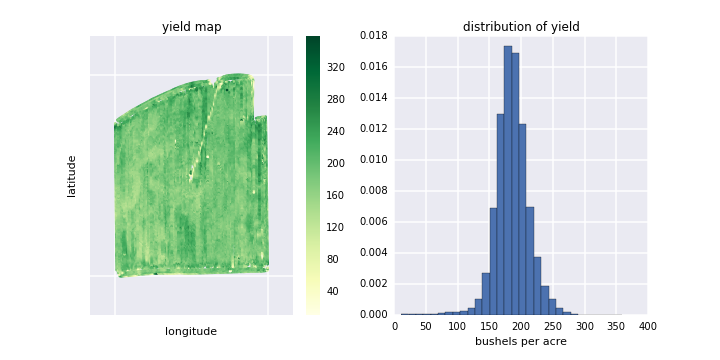
\includegraphics[width=15in]{figures/raw_data}
\caption{A yield map with the raw data and the distribution of yield at all measured locations}%
\label{fig:county_yield}
\end{center}
\end{figure}

The data come from a corn field in Butler County, Nebraska that was planted and harvested in 2009. Measurements are logged by a grain yield monitor which is connected to sensors on the arms of the tractor as it harvests corn. The yield monitor records an estimate of yield in bushels per acre and geolocation approximately six times per second. This results in $N = 16,898$ points. Using rejection sampling, the number of acres is found to be approximately 63.7.
% \begin{figure}
% \begin{center}
% 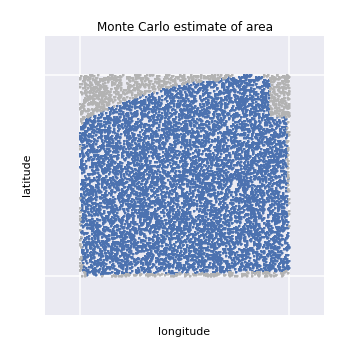
\includegraphics[width=7.5in]{figures/mc_area}
% \caption{Monte Carlo estimate of field area}%
% \label{fig:mcarea}
% \end{center}
% \end{figure}

\section{Method}

The importance sampling procedure for estimating yield consists of four steps:
\begin{enumerate}
\item Collect a small number of samples from $f(.)$
\item Construct the proposal function $g(.)$
\item Sample from $g(.)$
\item Use the samples to estimate yield
\end{enumerate}

A Gaussian Process is a distribution over functions and, assuming the mean is set to zero, is fully specified by a covariance kernel, $K(x_i, x_j)$ \cite{rasmussen}. One common form for the covariance function is a squared exponential: $$\sigma^2 \exp{\left(-\|x_i - x_j\|^2 / \phi\right)}$$ Assuming we know the hyper-parameters, $\sigma^2$ and $\phi$, we now have a function that we can use for importance sampling: $$g(x_{new}) = K(x_{new}, X)K^{-1}(X,X)y$$ which corresponds to the mean of the GP. Here, $X$ is the vecotor of locations for the $N_1$ samples and $x_{new}$ is the location of any arbitrary new point.

\begin{figure}
\begin{center}
  \begin{subfigure}[b]{6.75in}
    \centering
    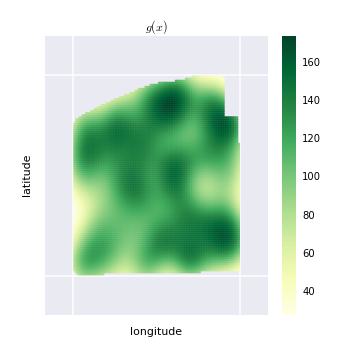
\includegraphics[width=\linewidth]{figures/gp}
    \caption*{Mean of GP}%
    \label{fig:resids_lat}
  \end{subfigure}
  \begin{subfigure}[b]{6.75in}
    \centering
    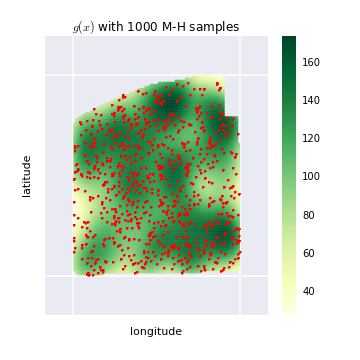
\includegraphics[width=\linewidth]{figures/gp_samples}
    \caption*{MH samples}%
    \label{fig:resids_lon}
  \end{subfigure}
\label{fig:test}
\end{center}
\caption{GP with Metropolis samples}
\end{figure}

Next, we can take $g(x)$ to be an unnormalized probability density and sample from it in order to find good candidate points for evaluating crop yield. I start with a simple Metropolis-Hastings sampler with symmetric proposals $q(x^{*}|x) \sim \mathcal{N}(x, \gamma)$, where $\gamma$ is set to 0.002 \cite{chib}.

\begin{figure}
\begin{center}
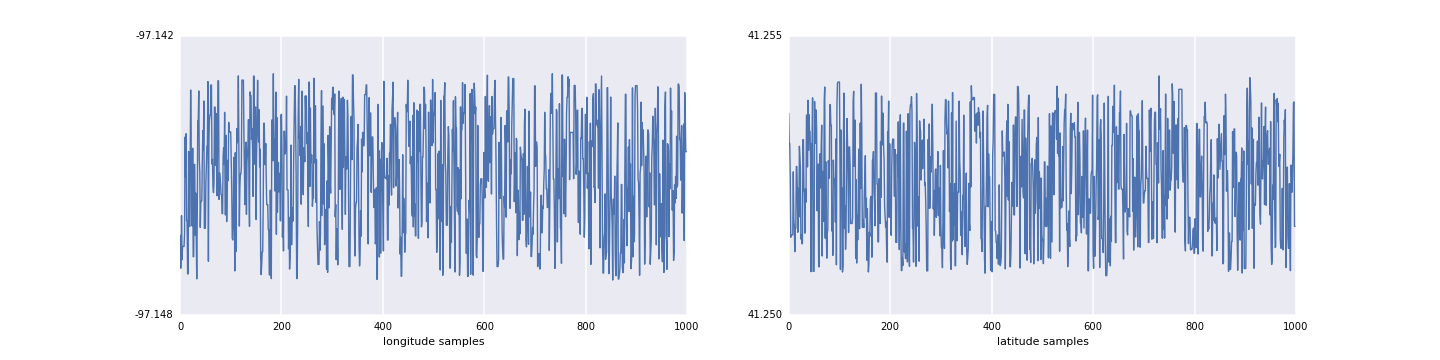
\includegraphics[width=15in]{figures/trace}
\caption{Trace plots of longitude and latitude samples from the M-H algorithm}%
\label{fig:mh}
\end{center}
\end{figure}

\section{Results}

Unsurprisingly, as the number of M-H draws increases, the the variance of the estimate decreases. Table \ref{tab:results} show the average estimate and the standard deviation of those estimates for $N_mc = 100, 500$, and $1,000$. Each experiment was performed 100 times. The left panel of Figure \ref{fig:results} shows histograms of the three levels of M-H draws and the right panel shows a box plot of the estimates and variance.

\begin{table}[H]
\begin{center}
\caption{Results}%
\begin{tabular}{rcr}
\hline
% {Model} & {parameters}  &  \shortstack{effective \\ parameters} &     $R^2$ &     RMSE \\
$N_{mc}$ & Bushels &  $\textrm{sd}(\hat{I}_{is})$ \\
\hline
100   & 11,987 & 160 \\
500   & 11,979 & 79 \\
1,000 & 11,988 & 58\\
\hline
\end{tabular}
\label{tab:results}
\end{center}
\end{table}

\begin{figure}
\begin{center}
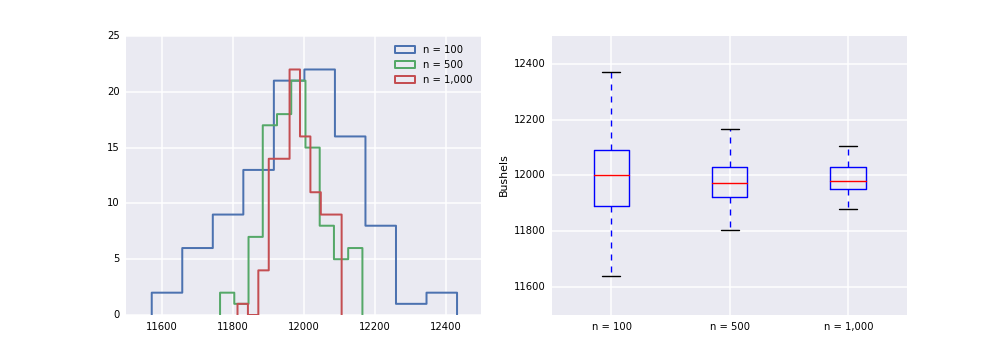
\includegraphics[width=15in]{figures/results}
\caption{Distribution of estimates of $|\Omega|\hat{I}_{is}$ and variance of estimate as the number of Metropolis samples increases}%
\label{fig:results}
\end{center}
\end{figure}

In practice, how many M-H samples need to be drawn would have to be determined by the farmers and agronomists who use this procedure. Samples are relatively expensive in the sense that each one needs to be collected by hand. 
Fortunately, even with only $N_{mc}= 100$ samples, the standard deviation of 160 is less than 2 \% of the number of bushels. This low variance makes the importance sampling method practical for estimating yield in real situations.



\section{Conclusions}

Stochastic optimization provides an important set of tools for estimating the crop yield in irregularly shaped fields. Fitting a GP to a few samples and then drawing several more importance samples from this proposal function decreases variance of estimated crop yield. This procedure can be used in a prediction setting with one additional step: by modeling how physical characteristics of the plant throughout the growing season drive yield at harvest.

% \cite{UDSA}
% \cite{CSRL}
% \cite{USHCN}

% \subsection{Problem Statement}
% \textbf{\large {\color{harvardcrimson} What spatial factors affect crop yield across the US?}}

% \section{Modeling Choices and Feature Selection}%
% We begin with a simple linear model, using features from climate, soil, and historical yield:

% \begin{align*}
%   y_{j,t} = & \beta_{0} + \beta_{1} t + \beta_{2} \overline{GDD}_{j,t} + \beta_{3} \overline{GDD}^{2}_{j,t} + \\
%   & \beta_{4} Prcp1_{j,t} + \beta_{5} Prcp2_{j,t} + \beta_{6} SW_{j}+ \epsilon_{j,t}
% \end{align*}

% The time feature in years allows us to represents the technology trend directly in the model. For climate features, we aggregate data from the 5 nearest weather stations to each county centroid. We define growing degree days as $GDD = max \left( 0, \frac{T_{max} - T{min}}{2} - T_{base} \right)$, where $T_{base}=10$. \cite{Bornn}  For precipitation, we take the first 2 bases of a non-negative matrix factorization performed on daily precipitation data (Prcp1-2) from each growing season from April 1 to October 31. Finally, we include an estimated soil water storage level (SW) measured in cm for each county.

% \begin{figure}
% \begin{center}
%   \begin{subfigure}[b]{.45\linewidth}
%     \centering
%     \includegraphics[width=\linewidth]{figures/lat_no_labels.png}
%     \caption*{Residuals vs Latitude}%
%     \label{fig:resids_lat}
%   \end{subfigure}
%   \begin{subfigure}[b]{.45\linewidth}
%     \centering
%     \includegraphics[width=\linewidth]{figures/lon_no_labels.png}
%     \caption*{Residuals vs Longitude}%
%     \label{fig:resids_lon}
%   \end{subfigure}
% \label{fig:test}
% \end{center}
% \caption{Simple Linear Model Residuals}
% \end{figure}

% The least squares model is too simple to capture the spatial variability that exists in the data. The above plots show residuals by longitude and by latitude. There are a number of ways to account for spatial dependence between counties. One simple approach is to fit a separate linear regression model to each state. Unfortunately, this approach results in overfitting, which hurts the predictive performance of the model.

% \subsection{MCAR}
% To account for spatial variability, we use a multivariate conditional autoregressive prior on the coefficients $\beta$ with:

% \begin{align*}
%   p(\beta) &= \mathcal{N}(0, \Lambda^{-1})  \\
%   \Lambda &= (D - \alpha W) \otimes \mathbb{I}
% \end{align*}

% $W$ is a $(6 \times 6)$ adjacency matrix that describes the neighborhood structure of states. We assign an edge to states that share a border. $|\alpha| < 1$ is a spatial smoothing parameter, and $D=diag(m_i)$, where $m_i$ is the sum of neighbors for state $i$. The right hand side of the kronecker product is required to be a positive definite matrix and we use the identity matrix for simplicity \cite{Jin}. \\


% \subsection{Numerical Stability}
% To avoid inverting the large matrices involved in the parameter estimation, we (1) specify the precision matrix directly and (2) use QR decomposition to compute the MAP estimate $\hat{\beta}_{\textrm{MAP}} = R^{-1}Q\widetilde{y}$, using: \cite{Murphy}\\
% % [-2ex]
% \setlength{\abovedisplayskip}{0pt}
% \begin{align*}
%   \widetilde{X} &= \left[ \begin{array}{c}
%                           X\\
%                           L
%                           \end{array}\right] 
%   & \widetilde{y} = \left[ \begin{array}{c}
%                          y\\
%                          \mathbf{0}
%                          \end{array} \right]\\
%   LL^T &= \Lambda & QR = \widetilde{X}\\
% \end{align*}
% where $R$ is easy to invert since it is upper triangular.

% % %\columnbreak

% \section{Results}
% \vspace{12pt}

% \begin{figure}
% \begin{center}
%   \begin{subfigure}[b]{.45\linewidth}
%     \centering
%     \includegraphics[width=\linewidth]{figures/rmse_mcar.png}
%     % \caption*{MCAR RMSE}%
%     \label{fig:rmse_mcar}
%   \end{subfigure}
%   \begin{subfigure}[b]{.45\linewidth}
%     \centering
%     \includegraphics[width=\linewidth]{figures/rmse_mls.png}
%     % \caption*{MLS RMSE}%
%     \label{fig:rmse_mls}
%   \end{subfigure}
% \label{fig:model-comparison}
% \caption{Model RMSE Comparison}
% \end{center}
% \end{figure}

% \vspace{12pt}


% \begin{wraptable}{l}{6in}
% \begin{table}
% \begin{center}
% \caption{Model Results}%
% \fontsize{32}{26.4}\selectfont
% \begin{tabular}{lcccc}
% \toprule
% % {Model} & {parameters}  &  \shortstack{effective \\ parameters} &     $R^2$ &     RMSE \\
% {Model} & $R^2$ &     RMSE \\
% \midrule
% Simple LS   & 0.44 & 42.96 \\
% LS by State & 0.50 & 65.36 \\
% MCAR        & 0.50 & 26.11 \\
% \bottomrule
% \end{tabular}
% \label{tab:model-results}
% \end{center}
% \end{table}
% \end{wraptable}
% After performing cross-validation we find that the spatial parameter that minimizes the RMSE is $\alpha = -0.25$. The above image shows that the MCAR regression model does not completely account for the spatial dependence, but it does dramatically better than fitting multiple least squares models.
% \vspace{12pt}

% \section{Conclusions}

% \begin{wrapfigure}{r}{8in}
% \begin{figure}
% \begin{center}
% \includegraphics[width=8in]{figures/predictions.png}
% \caption{Predictions with MCAR MAP estimate}%
% \label{fig:predictions}
% \end{center}
% \end{figure}
% \end{wrapfigure}

% In order to effectively model crop yield over a large area, we need to model the spatial dependence between locations. The MCAR model reduces the effects of overfitting apparent in the multiple least squares model grouped by states and exhibits significantly lower RMSE than either of the least squares models.

% \vspace{12pt}
{\footnotesize
  \bibliography{sample}
}
% \vspace{12pt}

% \subsection{Acknowledgments}

% Thanks to Luke Bornn for critical recommendations and insights.

\end{poster}

\end{document}


